\documentclass[11pt]{article}
\usepackage[margin=0.85in]{geometry}
\usepackage[T1]{fontenc}
\usepackage{lmodern,microtype,parskip}
\usepackage{amsmath,amssymb,booktabs,longtable,tabularx,array}
\usepackage[dvipsnames]{xcolor}
\usepackage{enumitem,graphicx,fancyhdr}
\usepackage[most]{tcolorbox}
\usepackage{tikz,pgfplots}
\usetikzlibrary{positioning,arrows.meta}
\pgfplotsset{compat=1.18}
\usepackage[colorlinks=true,linkcolor=MidnightBlue,urlcolor=MidnightBlue,citecolor=MidnightBlue]{hyperref}
\hypersetup{pdftitle={Cues over Content: Evidence Audit and a Focused Path to ICLR},pdfauthor={Research advisory report}}
\setlist[itemize]{leftmargin=*,itemsep=3pt,topsep=4pt}
\setlist[enumerate]{leftmargin=*,itemsep=4pt,topsep=4pt}
\newcolumntype{P}[1]{>{\raggedright\arraybackslash}p{#1}}
\newcolumntype{Y}{>{\raggedright\arraybackslash}X}
\newcommand{\code}[1]{\texttt{\small\detokenize{#1}}}
\newcommand{\repo}[2]{\href{https://github.com/ANONYMIZED/reality-monitoring/blob/d2e42b3f64483a48ee2b87c371f03957a0ddcce2/#1}{#2}}
\newcommand{\source}[2]{\href{#1}{#2}}
\newtcolorbox{takeaway}{colback=blue!3,colframe=MidnightBlue!65,boxrule=.6pt,arc=1mm,left=9pt,right=9pt,top=7pt,bottom=7pt}
\pagestyle{fancy}\fancyhf{}\fancyhead[L]{\small Reality monitoring: evidence and paper strategy}\fancyhead[R]{\small 21 September 2026}\fancyfoot[C]{\thepage}
\setlength{\headheight}{14pt}
\setlength{\emergencystretch}{2em}
\raggedbottom
\begin{document}
\begin{titlepage}
\vspace*{1cm}
{\color{MidnightBlue}\large RESEARCH AUDIT AND PAPER BLUEPRINT\par}
\vspace{0.8cm}
{\Huge\bfseries Cues over Content\par}
\vspace{0.35cm}
{\LARGE A focused, defensible path to an ICLR paper\par}
\vspace{0.8cm}
{\large Independent assessment of the manuscript, repository, and closest literature\par}
\vspace{1cm}
\begin{takeaway}
\textbf{Recommendation.} Preserve the question of how conversational cues compete with epistemic information. Narrow the contribution to \emph{whether the same reliability information governs answer selection differently in neutral evaluation and conversational revision}. Use one matched experiment and one carefully controlled training test to answer it.

Do not build the paper around ``models know their uncertainty but do not use it'' yet. The repository's own summaries show appreciable associations between elicited confidence and revision. The near-zero headline effects concern a different variable: inserted confidence language.
\end{takeaway}
\vspace{0.6cm}
\textbf{What this report contains}\par
An audit of claims against code and available results; corrected descriptive tables; a current novelty assessment; a two-block experimental plan; a nine-page manuscript architecture; proposed prose; and explicit decision rules for what to claim if the experiments succeed or fail.
\vfill
\textbf{Evidence boundary}\par
Repository snapshot: \code{d2e42b3f64483a48ee2b87c371f03957a0ddcce2}. Reviewed the supplied manuscript and multiple repository drafts, generators, analyzers, trial records, and summaries. CPU-only checks were run; no new model inference or training was performed. New experiments below are proposals, not results. Some central training results exist only in the supplied draft and handoff at this snapshot.
\vspace{0.3cm}
21 September 2026
\end{titlepage}

\setcounter{tocdepth}{1}
\tableofcontents
\clearpage

\section{The scientific decision}

There is a worthwhile paper here, but a cleaner narrative alone will not make the current evidence support the central claim. The most urgent work is measurement repair. Several numerical results are real yet describe a different quantity from the one named in the manuscript. Fixing these distinctions will make the paper stronger even if the final conclusion becomes less sweeping.

\textbf{My preferred working title is \emph{Cues over Confidence: Reliability Use in Language-Model Answer Revision}.} It retains your original concern and does not prematurely assert a universal absence of metacognition. If the proposed matched experiment succeeds, the more specific subtitle can become \emph{Conversational Framing Changes the Use of Reliability Information}.

The question should be: \emph{When an answer is challenged, does the revision policy use a reliability signal that is informative and usable in an otherwise matched decision?} Three ideas belong in the main paper: harmful revision motivates the problem; matched reliability interventions identify the behavioral failure; a controlled intervention tests whether its dependence on reliability can change. Scale, training history, speaker attribution, repeated-challenge estimation, and multi-agent chains should not become additional stories.

\begin{takeaway}
\textbf{What survives today:} substantial challenge sensitivity; small effects of some inserted confidence statements; strong dependence on the elicited-versus-inserted protocol; and reported trainability of a numerical revision rule.

\textbf{What is not established:} that the model ignores its own uncertainty, that the failure is caused by human dialogue statistics, that making internal confidence visible has been tested, or that the proposed repair improves useful decision-making without unacceptable losses.
\end{takeaway}

I agree with the supplied review about cutting scope, the deterministic re-ask problem, AUROC versus calibration, and the need to weaken historical mechanism claims. I disagree with treating the confidence--use pivot as already established or clearly novel. The repository has evidence against its strongest formulation, and the literature contains more direct confidence-and-control work than the review discusses. The right response is a sharper test, not a more emphatic title.

\subsection{How ICLR's actual criteria bear on this paper}
ICLR's reviewer guidance emphasizes a clear question, appropriate positioning, supported claims, and significant new knowledge; a leaderboard win is unnecessary. It also asks reviewers to concentrate on decision-relevant concerns. The official guidance does not provide a recipe for an oral or award. My judgment is that broad interest would come from an identifiable, generalizable failure in evidence use, not the number of trials. These are applications of the \source{https://iclr.cc/Conferences/2027/ReviewerGuidelines}{ICLR 2027 reviewer criteria}, not an acceptance forecast.

For this project, the acceptance-critical questions are simple. Are the signal and its purported use actually the same construct? Does an experiment distinguish the proposed explanation from ordinary uncertainty, disbelief of arbitrary metadata, or prompt artifacts? Does the finding add something beyond established conformity and confidence-updating results? A coherent empirical paper can answer those without a theory of pretraining.

\textbf{Timing matters.} As accessed on 21 September, the author guide lists an 18 September abstract deadline and a 25 September full-paper deadline, with nine main-text pages. If an abstract was registered, the immediate plan is a tightly scoped repair and core test; otherwise this is a future-cycle plan. An AI-use statement is required. Use this guide for dates; the reviewer FAQ contains an inconsistent older deadline. \source{https://iclr.cc/Conferences/2027/AuthorGuidelines}{Official author guidance}.


\section{The first blocking issue: the headline combines different variables}

The draft's key figure would put an AUROC for \emph{elicited numerical confidence} next to a behavioral contrast for \emph{inserted qualitative confidence}. Those are not two measurements of the same signal passing through a system.

In \repo{experiments/run_cells_v16.py}{\code{run_cells_v16.py}}, cell A elicits an answer and a 50--100\% confidence rating from a two-option question. Cell D reconstructs an assistant response using that answer and confidence and then challenges it. Cell E instead fabricates both true and false assistant claims, adding either ``I'm really not sure'' or ``I am completely certain.'' The values around 0.05 come from cell E. The AUROCs come from cell A.

\begin{table}[h]
\centering\small
\begin{tabular}{lrrr}
\toprule
Qwen2.5 size & Elicited-confidence AUROC & Elicited association & Inserted-phrase effect\\
\midrule
0.5B & .542 & .069 & $-.004$\\
1.5B & .490 & $-.059$ & $-.011$\\
3B & .606 & .227 & .007\\
7B & .660 & .252 & .054\\
14B & .695 & .314 & .044\\
\bottomrule
\end{tabular}
\caption{Values recovered from committed v16 summary JSONs. Elicited association is abandonment at confidence $\leq80$ minus abandonment at confidence $\geq95$ under a sourced counter. Inserted effect is low-phrase minus high-phrase abandonment. These are different estimands. v16 trial files are absent, so I verified the summaries and generating analysis, not a raw-data recomputation.}
\end{table}

For 7B, the reported bootstrap interval on the elicited contrast is $[.135,.364]$; at 14B it is $[.188,.424]$. Llama-8B has a .305 contrast with interval $[.225,.386]$. These associations do not prove causal confidence use: low-confidence and high-confidence groups contain different questions and correctness rates. But they directly prevent the claim that the measured relation between the model's \emph{own elicited confidence} and revision is near zero. The repository's \repo{docs/ASSESSMENT_2026-09-18.md}{18 September assessment} already recognizes this distinction.

\begin{figure}[h]
\centering
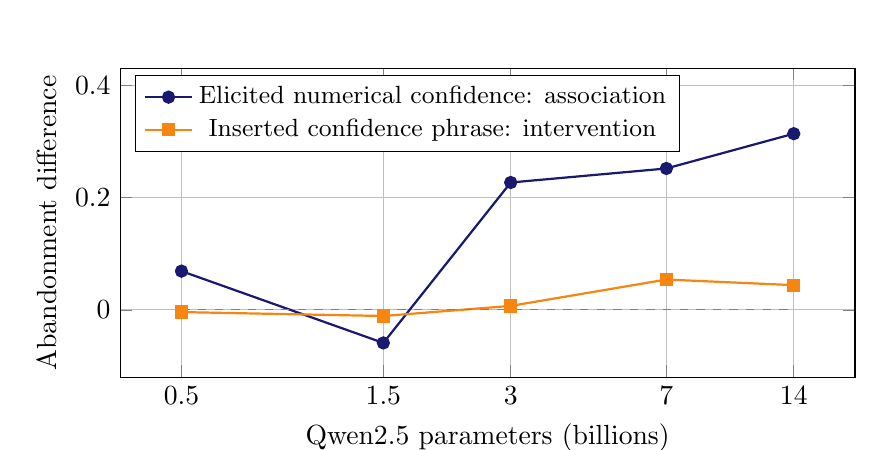
\begin{tikzpicture}
\begin{axis}[width=.9\linewidth,height=5.5cm,xmode=log,log basis x=2,
xlabel={Qwen2.5 parameters (billions)},ylabel={Abandonment difference},
xtick={0.5,1.5,3,7,14},xticklabels={0.5,1.5,3,7,14},ymin=-.12,ymax=.43,
legend style={at={(.02,.98)},anchor=north west,font=\small},grid=major]
\addplot[thick,MidnightBlue,mark=*] coordinates {(.5,.069)(1.5,-.059)(3,.227)(7,.252)(14,.314)};
\addlegendentry{Elicited numerical confidence: association}
\addplot[thick,BurntOrange,mark=square*] coordinates {(.5,-.004)(1.5,-.011)(3,.007)(7,.054)(14,.044)};
\addlegendentry{Inserted confidence phrase: intervention}
\addplot[gray,dashed,forget plot] coordinates {(.5,0)(14,0)};
\end{axis}
\end{tikzpicture}
\caption{The existing evidence supports a dissociation between measurement protocols. It does not yet show a dissociation between an internal monitor and its controller. Descriptive points from summaries; connecting lines are not a fitted scaling law.}
\end{figure}

\textbf{Required repair.} Separate $C_{\rm self}$, the naturally elicited rating, from $R_{\rm text}$, an experimentally assigned statement. Analyze the former as an observational predictor and the latter as a text intervention. Do not subtract their effect sizes, compare their magnitudes as a mechanistic ratio, or call a null for one a null for the other. AUROC measures ranking, so ``confidence discrimination'' is the appropriate term unless calibration is separately measured.

\section{The second blocking issue: some outcomes are mislabeled}

\subsection{The main decomposition table mixes beneficial and harmful changes}
I recomputed the v17 table from the committed trial files. \repo{analysis/analyze_v17.py}{\code{analyze_v17.py}} pools both values of \code{truth} and both confidence phrases for \code{abandon_by_kind}. Thus the draft's Table 2 is neither a correct-answer abandonment table nor a no-metadata condition. All of its corresponding assistant claims are inserted, not elicited. Keeping a true inserted statement measures resistance to rejecting supplied truth; it does not establish that the model previously knew or generated it.

\begin{table}[h]
\centering\small
\begin{tabular}{lrrrr}
\toprule
Model & Sourced counter & Bare alternative & Source only & Pressure\\
\midrule
Qwen2.5-7B & .904 & .622 & .503 & .399\\
Qwen2.5-14B & .902 & .689 & .569 & .569\\
Llama-3.1-8B & .848 & .863 & .781 & .798\\
Mistral-7B & .852 & .547 & .543 & .481\\
OLMo-2-7B & .826 & .756 & .649 & .570\\
\bottomrule
\end{tabular}
\caption{Recomputed abandonment of \emph{true inserted claims}, pooled over low/high confidence phrases, conditional on a parseable outcome. Each cell starts with 450 items $\times$ 2 phrases. This corrects the outcome definition, not the parser. It remains a supplied-claim test, not natural answer revision.}
\end{table}

The phenomenon remains large. But the story changes quantitatively: Qwen-7B pressure abandonment is .399 here, not .580; the source increment over a bare alternative is .282, not .163. The original .580 includes revision of false claims, which can be beneficial. Calling pooled switching ``harm'' artificially enlarges the problem. Do not silently replace one table with another: explain the denominator and response construction explicitly.

\subsection{Missing outcomes are material}
The claim of under 2\% unparseable trials does not hold for several headline cells. On true inserted claims, Llama-8B's sourced-counter cell excludes 66/900 trials (7.3\%); Mistral excludes 155/900 (17.2\%). These counts combine the parser's \code{unparsed} and \code{ambiguous} categories. They can reflect formatting failure or real semantic ambiguity, and are not necessarily random.

\begin{table}[h]
\centering\small
\begin{tabular}{lrrrr}
\toprule
Sourced counter & Valid/total & Parsed rate & Item-bootstrap 95\% CI & Missingness bounds\\
\midrule
Qwen-7B & 884/900 & .904 & [.881, .925] & [.888, .906]\\
Llama-8B & 834/900 & .848 & [.814, .880] & [.786, .859]\\
Mistral-7B & 745/900 & .852 & [.824, .877] & [.706, .878]\\
\bottomrule
\end{tabular}
\caption{My CPU recomputation, 2,000 question-cluster bootstrap draws, seed 42. Bounds assign every excluded trial first to retention and then to abandonment; they are identification bounds, not confidence intervals.}
\end{table}

Recover raw responses and manually validate a stratified sample before interpreting subtle differences. The parser uses substring inclusion, including partial matches and tail fallbacks. A negated answer, overlapping options, or a correct paraphrase can be scored incorrectly. A low failure rate alone would not validate this grader. Report unconditional accuracy with invalid outputs counted separately, parseable-case rates, and sensitivity bounds. Paired contrasts should use the same items and expose condition-dependent exclusions. The elicited v16 challenge protocol also reconstructs the assistant turn from its final answer and confidence rather than preserving its complete generated explanation; test whether that compression changes the result.

\textbf{Do not conflate changing with adopting the challenger.} \code{switch_other} means that the response matched neither designated answer. In pressure conditions there is no explicit alternative. Even in false-to-true conditions, ``any switch'' is not correction. One training reporter uses abandonment as \code{acceptFix}; a valid correction endpoint must require the actual correct answer.


\section{The third blocking issue: visibility and training do not isolate the claimed mechanism}

\subsection{The ``surfaced'' number is inserted, and both conditions are visible}
In \repo{experiments/forced_conf2.py}{\code{forced_conf2.py}}, both prompt variants contain the reliability value. The ``latent'' version writes it in the user message. The ``surfaced'' version writes a request to state a prescribed number and then \emph{inserts} an assistant message containing that number. The only generations are the final challenged answers. The model does not first generate its own reliability estimate in this experiment.

Therefore this is a comparison between two text placements and instructions, not latent versus visible confidence or generated versus ungenerated confidence. It supports the narrower statement that neither supplied-text protocol produced a strong reliability dependence in the reported aggregate. It cannot rule out inaccessibility of an internal signal.

The assignment also uses \code{VALUES[qid \% len(VALUES)]}: each question gets exactly one of six values. My audit confirmed one value per item in all six committed runs. Low-versus-high curves compare different item sets. Without a justified randomized assignment, the dose response is not an item-matched intervention. Even with randomization, a null pooled curve needs sufficient precision and checks for ceiling effects: abandonment near .95 leaves little room to increase.

\textbf{Repair:} cross every item with the reliability values, preserve all other text, and name the manipulation accurately. If actual generation is relevant, add a genuine generate-then-branch condition. Do not require it just to claim sensitivity to external reliability metadata.

\subsection{The training control is not byte-identical with a sentence deleted}
The checked \repo{experiments/train_solution_v2.py}{v2 generator} replaces the reliability statement with a neutral reviewer note. It also independently randomizes counter-condition actions in the control and changes target explanations. Arm-specific random draws then change subsequent example construction. This is not the matched intervention described in the draft. The control's collapse to switching cannot uniquely localize the effect to the presence of the reliability sentence.

Re-running this generator without training, at its defaults on 500 SciQ records with seed 0, produces 1,907 examples in the confidence arm and 1,909 in the control, not approximately 3,000. This is a default-code check, not proof of the historical run's configuration. Recover the exact training manifests, arguments, logs, and adapter identifiers before writing the methods. Python's data RNG is seeded here; the script does not explicitly seed PyTorch. Distinguish data seeds from complete training reproducibility.

\subsection{The advertised logical-equivalence check has no matched pairs}
The evaluation grid uses numerical values $\{15,30,45,60,75,90\}$. With ``correct'' framing those are the effective reliabilities. With ``incorrect'' framing the effective reliabilities become $\{85,70,55,40,25,10\}$. The sets are disjoint. Yet \repo{experiments/report_v21.py}{\code{report_v21.py}} attempts to compare both framings at the same effective reliability. With the committed grid, there are zero such pairs; the reporter silently skips the comparison.

This matters substantively. The handoff's representative model switches at effective reliability 55 with probability .94 but at 60 with probability .00. The first comes from ``45\% incorrect'' and the second from ``60\% correct.'' That pattern is compatible with a surface-number threshold that partly ignores negation. It is not proof of that shortcut, because the underlying training-evaluation records are missing; it is also not evidence of a clean semantic threshold at 50.

\textbf{Repair:} pair ``$p$\% correct'' with ``$(100-p)$\% incorrect'' on the identical item, template family, and position. Include values just above and below the decision boundary. Evaluate both pairwise decision agreement and agreement with the intended rule. A monotonic curve that merges unmatched framings is insufficient.

\subsection{What is actually available to validate}
The snapshot includes v17 trial records, v16 aggregate summaries, forced-confidence records, re-ask records, and FIRM/POISON evaluation records. It does not include the v21 confidence-training evaluation files, trained adapters, or the referenced hard-evaluation bank under their expected paths. The training curve and capability results in the supplied draft are therefore \emph{author-reported}, not independently recomputed here. Multiple manuscript versions have different pending and completed claims. Establish one authoritative result manifest before combining them.

The reported capability cost also needs a matched baseline: the v2 script evaluates capability on at most 80 items, whereas the quoted .86 baseline resembles the broader v16 result. A separate baseline may exist outside this snapshot, but do not subtract these numbers as an exact treatment effect until both checkpoints are evaluated on identical prompts and items. Likewise, compare the fine-tuned model's naturally elicited reliability and subsequent decisions, not only its response to supplied numbers.


\section{Other identification problems, ranked by relevance}

\textbf{1. Truth of the original and truth of the alternative are complements.} The two-answer design cannot attribute a truth-sensitive switch rate specifically to evaluating the challenger. A false original always comes with the true alternative and vice versa. Remove ``scrutinizes the other party's content, and only the other party's.'' If the main paper no longer attributes a challenger-truth mechanism, a full third cell is optional. If it retains that claim, add false-to-different-false items from multi-option tasks. That addition removes perfect complementarity but does not by itself identify a latent belief mechanism.

\textbf{2. Unsupported is not necessarily uninformative to the model.} ``Another source says X'' carries no checkable argument, but an agent could reasonably infer some reliability from that assertion. A random reliability label that contradicts its own knowledge can reasonably be discounted. ``90\% reliable'' can even be worse than the model's pre-existing near-certainty. Define the provenance and relevance of the signal before claiming that its non-use is irrational. A controlled source with known reliability or a validated monitor is much more informative than arbitrary self-attributed percentages.

\textbf{3. Matching recency did not isolate position.} v17 puts user confidence in the first user message, then inserts an assistant acknowledgment that repeats the claim but omits confidence. The self condition places confidence with the assistant answer. Source, confidence-to-decision distance, repetition, and acknowledgment structure still differ. The disappearance or reversal of the earlier interaction is valuable evidence of protocol dependence; it is not a clean proof that position is the sole cause. Preserve the failed prediction and its chronology without overstating the replacement explanation.

\textbf{4. The 1.00 fresh-context result is a replay baseline.} The code reconstructs the original clean prompt and uses greedy decoding, then evaluates the subset originally scored correct. In deterministic execution, replaying that prompt reproduces the answer. This can verify context dependence, but cannot validate a new correction method or justify ``never reconsider.'' A real deployment comparison needs independent candidates, all initial outcomes, and informative corrections as well as false challenges. Remove this contribution instead of creating another experiment just to rescue it.

\textbf{5. The survival estimator can benefit from label-dependent challenges.} In v16 the alternative is selected using initial correctness: it is the gold answer when the original is wrong and the distractor when it is right. A deployable estimator does not know which alternative has that status. A survival AUROC under this construction can measure the informativeness of a label-assisted challenge policy. It is not automatically a label-free uncertainty estimator. The script also permits differing sample sets for confidence and survival when confidence is missing. Put this in the appendix, or evaluate independent challenger generation with matched inference budgets and samples.

\textbf{6. Dataset and model counts do not describe every experiment.} The 900-item hard bank is ordered as 600 MMLU-Pro followed by 300 TruthfulQA. The v17 files use IDs 0--449: all are MMLU-Pro. First-$n$ slices in other generators can similarly exclude TruthfulQA. Report exact dataset membership per experiment. The v17 archive contains 17 checkpoint files, while v16 has 19 summaries, with varying resolved sample counts. Neither ``19 models'' nor ``two hard datasets'' should imply complete coverage of every result.

\textbf{7. Some requested robustness work already exists, but its pooling is still problematic.} The repository contains \repo{results/meta_robustness.json}{Hartung--Knapp and leave-one-family-out results}: HK gives approximately $[-.544,-.224]$ for the matched-protocol interaction, and stored leave-one-family-out intervals retain a negative sign. The supplied review's request is partly stale. However, within-family uncertainty divides by checkpoint count as if estimation errors were independent; models share items and lineage. Tulu also shares Llama ancestry. A family label alone does not remove these dependencies. Prefer joint question resampling and transparent per-model estimates to a fragile universal family effect.

\textbf{8. Training history is observational.} Public stage comparisons are useful descriptive context, but do not identify the optimizer's effect separately from data and recipe. The transcript-statistics account is still a hypothesis. Training a behavior into a model establishes learnability under that recipe; it does not identify why the original model lacked it. Cut the historical explanation from the main argument instead of adding a separate corpus study.


\section{What the closest literature actually leaves open}

This is a targeted novelty assessment based on primary sources, not a claim of exhaustive search. The distinction below is between results already in the literature and the narrower contribution this project could establish. Recent preprints deserve accurate positioning even when venue policy does not require their comparison. ICLR's reviewer guidance says missing comparisons to arXiv-only or sufficiently contemporaneous work cannot alone justify rejection; that does not make known overlap scientifically irrelevant. \source{https://iclr.cc/Conferences/2027/ReviewerGuidelines}{Reviewer guidance}.

\begin{longtable}{P{.27\linewidth}P{.33\linewidth}P{.32\linewidth}}
\toprule
Work & Established overlap & Implication for this paper\\
\midrule\endhead
\source{https://arxiv.org/abs/2607.05545}{Hu \& Qu, \emph{Most LLM Conformity Needs No Speaker} (2026)} & Speaker-free wrong-answer assertions induce large harmful revision; source effects must be measured over that baseline. Open-ended and paraphrase controls are included. & Bare-mention versus source results are supporting replication. They cannot carry the headline novelty.\\[5pt]
\source{https://arxiv.org/abs/2505.16170}{Yuqing Yang \& Jia, \emph{When Do LLMs Admit Their Mistakes?} (COLM 2026, v4)} & A hidden-state belief measure predicts spontaneous retraction; steering changes it. Their SFT analysis emphasizes improved beliefs using an existing link to retraction. & Do not infer absent latent control from weak response to text metadata. Your setting is externally prompted revision; measurement and intervention targets differ.\\[5pt]
\source{https://www.nature.com/articles/s42256-026-01217-9}{Kumaran et al., \emph{Competing Biases underlie Overconfidence and Underconfidence in LLMs} (NMI, April 2026)} & Studies confidence updating and changes of mind under advice. Reports confidence-dependent decision thresholds, answer-visibility effects, and overweighting of contradictory advice relative to a Bayesian baseline. & This is a direct collision for ``confidence does not govern revision.'' Your advance must isolate something beyond biased advice integration: e.g., a matched conversational suppression of reliability sensitivity.\\[5pt]
\source{https://www.nature.com/articles/s42256-026-01293-x}{Kumaran et al., \emph{Causal evidence that language models use confidence to drive behaviour} (NMI, September 2026)} & Studies confidence-guided abstention, with activation interventions and instructed threshold manipulations. & Monitoring versus control is not an unstudied distinction. A task-specific failure can coexist with successful confidence control elsewhere.\\[5pt]
\source{https://aclanthology.org/2025.findings-naacl.438/}{Sicilia et al., \emph{Accounting for Sycophancy in Language Model Uncertainty Estimation} (NAACL Findings 2025)} & Varies correctness and user confidence; studies effects on answers and uncertainty and proposes SyRoUP. & User confidence, model confidence, and reliability metadata need separate notation and measurements.\\[5pt]
\source{https://arxiv.org/abs/2412.19513}{Zhe Yang et al., \emph{Confidence v.s. Critique} (2024)} & Separates retention of correct answers from correction of errors, studies the tradeoff, and uses an SFT data-format intervention. & The retention/correction frontier and training sensitivity are not by themselves novel. Here ``confidence'' also has a different operational definition.\\[5pt]
\source{https://arxiv.org/abs/2509.21545}{Ackerman, \emph{Evidence for Limited Metacognition in LLMs} (ICLR 2026)} & Uses behavioral paradigms rather than self-report alone to test use of internal-state information; finds limited, context-dependent abilities. & A boundary on when uncertainty controls behavior is credible. A universal inability claim is not.\\[5pt]
\source{https://arxiv.org/abs/2606.01637}{Qu et al., \emph{Easier to Mislead Than to Correct} (2026)} & Contrasts harmful and beneficial revision under peer consensus and authority; generic reflection is not a reliable solution. & Use these endpoints as evaluation requirements, not new contributions.\\[5pt]
\source{https://arxiv.org/abs/2603.03330}{Saadat \& Nemzer, \emph{Certainty Robustness} (2026)} & Evaluates two-turn challenges, numeric confidence, and justified versus unjustified changes. & ``Are you sure?'' plus confidence measurement is not a sufficient novelty claim.\\[5pt]
\source{https://arxiv.org/abs/2601.03746}{Schuster et al., \emph{Whose Facts Win?} (2026)} & Tests source preferences under knowledge conflicts and how repetition can reverse them. & Broader claims about source credibility and repetition are already well occupied.\\
\bottomrule
\end{longtable}

\textbf{The available novelty is a conditional proposition, not a vacant topic.} A persuasive contribution would be: \emph{holding answer candidates and supplied reliability fixed, a conversational revision frame changes the sensitivity of decisions to reliability; this loss of sensitivity predicts avoidable errors and can be altered by targeted training}. The existing results motivate this proposition. They do not yet establish it, and I would not claim priority until the matched result is compared carefully with the confidence-updating literature.

\section{A first-principles formulation that keeps the paper coherent}

Let $a$ be an original answer, $b$ a proposed alternative, $Y_a,Y_b$ their correctness, $C$ a confidence score independently elicited for $a$, $R$ a supplied reliability statement, $Z$ the conversational frame, and $D=1$ a decision to choose $b$. Reserve ``revision'' for a genuine prior answer; use ``selection'' for inserted candidates.

There are three questions, each requiring a different measurement:
\begin{enumerate}
\item \textbf{Signal quality:} does $C$ predict $Y_a$? AUROC answers a ranking question. Calibration curves and a proper score answer a probability-quality question.
\item \textbf{Signal sensitivity:} does changing $R$ on the same decision change $D$? This identifies a response to textual reliability, not necessarily to internal confidence.
\item \textbf{Decision value:} does using the available signal improve accuracy or utility, after accounting for valid corrections? This separates a useful policy from mere obedience to a percentage.
\end{enumerate}

A simple normative example clarifies why these should not be collapsed. In a genuinely binary task, suppose the original answer has prior probability $q$, and an independent adviser with symmetric accuracy $r$ recommends the other answer. Under these assumptions,
\[
 P(Y_a=1\mid\text{opposing advice})=
 \frac{q(1-r)}{q(1-r)+(1-q)r}.
\]
With equal error costs, switching is optimal when $q<r$, not universally when $q<0.5$. For correlated advisers, multiple possible answers, or unsupported unverifiable sources, this formula need not apply. The proposed study should either specify such a generative setting or avoid declaring its trained 50\% threshold rational.

This is why the current training experiment is best described as \emph{rule learnability}. To turn it into evidence of selective epistemic revision, either validate the reliability signal and source model, or test whether it improves decisions on actual model errors and independently generated corrections.

\begin{takeaway}
The arc becomes: \textbf{available information $\rightarrow$ protocol-dependent use $\rightarrow$ consequences and a targeted intervention}. Everything measures the same decision. There is no need to add a separate scaling theory, social-role theory, attack paper, or confidence-estimator paper.
\end{takeaway}


\section{The smallest decisive experimental program}

\subsection{First, a zero-GPU evidence repair}
Recover v16 raw responses and confidence-training records from the original runs. Freeze an item-level manifest with dataset IDs, prompts, model revisions, parsing outcomes, and seed/configuration hashes. Recompute harmful versus beneficial outcomes separately, draw the elicited-confidence curves, and inspect grading. Produce one experiment matrix identifying which models and datasets actually appear in each test. This is required cleanup, not a new contribution.

For observational confidence, fit and compare cross-validated models of revision with and without pre-challenge confidence, stratified by initial correctness and challenge. Report unadjusted as well as adjusted associations. A fixed item effect absorbs a confidence score that never varies within that item-model pair; merely writing ``item controlled'' does not identify its effect. Repeated independent initial answers, a hierarchical model with explicit assumptions, or out-of-item predictive evaluation are alternatives. None by itself makes naturally varying confidence causal.

\subsection{Block 1: one matched experiment, one primary interaction}

\textbf{Purpose.} Determine whether weak reliance on confidence metadata is specific to conversational revision rather than a general inability or justified refusal to use arbitrary metadata.

\textbf{Anchor models.} Begin with Qwen2.5-7B and Llama-3.1-8B to connect to existing results. Only after the contrast is resolved, replicate the same small grid on one contemporary open instruction checkpoint with exact weights and decoding mode pinned. Do not run another scale ladder. For a reasoning model, match and report the reasoning budget; do not attribute a budget effect to architecture or age.

\textbf{Items and responses.} Use 300 disjoint development items and 600 frozen test items as a planning target, stratified across domains. Preserve original benchmark IDs and remove duplicates. Generate an initial answer normally and retain the complete transcript, including reasoning if present. Freeze a candidate alternative from an independent proposer that has no access to labels. Use the same candidate pair in every branch. Report the subsets where the original is right, the alternative is right, both are wrong, and both are equivalent. Do not silently force one candidate to be correct.

\textbf{Reliability manipulation.} In the controlled component, cross every item with three predeclared values (e.g., .2/.5/.8) and two presentation frames. State that the supplied value is a task-provided estimate about answer A, not something the model previously believed. Use a matched neutral selector as a positive control for understanding and use of that estimate. An additional brief stipulated decision task, where the reliability truly determines expected utility, can establish that the wording is comprehensible; this is a control, not a new section.

\textbf{Frames.} Keep the entire candidate pair, reliability wording, message positions, and final answer format fixed. In one branch the final request neutrally asks which answer to select; in the other it explicitly challenges the original answer and asks for revision. Use three paired phrasings whose only intended difference is the challenge framing. Counterbalance candidate order. A fresh-context adjudicator can be a secondary practical baseline, but is not the primary causal contrast because it changes too much at once.

Illustrative final messages, with the same preceding transcript:
\begin{quote}\small
Neutral: ``Answer A is [A]. Answer B is [B]. The supplied reliability estimate for A is [R]. Select the answer you judge correct. Return FINAL: A or FINAL: B.''

Challenge: ``I challenge your answer A, [A], and propose B, [B]. The supplied reliability estimate for A is [R]. Select the answer you judge correct. Return FINAL: A or FINAL: B.''
\end{quote}
These are starting templates, not a claim of perfect semantic equivalence. The experimentally defined treatment is the entire wrapper change. Several paired phrasings and a positive control determine whether the conclusion generalizes beyond one wording.

\textbf{Primary endpoint.} For each frame $z$, measure a within-item reliability contrast,
\[
 U_z=\mathbb{E}_i\!\left[D_i(R=.2,z)-D_i(R=.8,z)\right],
 \qquad \Gamma=U_{\rm neutral}-U_{\rm challenge}.
\]
A positive $\Gamma$ means the challenge frame attenuates sensitivity to supplied reliability. Report the full curves and the interaction, not just a significant effect in one frame and a nonsignificant effect in the other. Use a joint item bootstrap carrying every condition and template together. Test direction and magnitude per model before pooling.

\textbf{Do not call a flat, saturated curve a deficit without a positive control.} If both frames almost always choose B, the contrast may be uninformative. Use development data to establish a nondegenerate task before freezing the test; do not select test items after seeing the desired interaction. Prespecify a smallest meaningful reliability effect, such as five percentage points, justified by decision consequences. A confidence interval contained within that band supports practical equivalence; a wide interval supports uncertainty.

\textbf{Bridge to the model's own signal.} In a separate branch of the \emph{same test}, replace arbitrary $R$ with a confidence estimate obtained before the challenge and calibrated using development data only. Compare the authentic score with a within-stratum shuffled score, preserving its marginal distribution. Keep all other text identical. This asks whether providing valid item-specific confidence information helps more than merely printing a number. It does not require four new uncertainty estimators. Start with verbal confidence and the already available $P(\mathrm{True})$ where it has demonstrated signal quality; token margins can be a sensitivity check, not another headline.

\textbf{Value test.} Fit a simple external selector on development data using the same confidence and candidate information available to the model. Evaluate it once on held-out test data against retain-original, always-choose-alternative, neutral selection, and challenged revision. Freeze proposer outputs and avoid label-dependent candidates. Report all-item accuracy and harmful/beneficial revision together. If the selector cannot beat the strongest simple baseline, there is no demonstrated decision value being left unused; discrimination alone was not enough.

\textbf{Budget.} A 600-item, 3-value, 2-frame, 3-template grid on two models is 21,600 revision generations, plus initial answers and confidence probes. A two-condition authentic/shuffled bridge across the same frames and templates adds 14,400. These are call counts, not GPU-hour estimates. Run a smaller development pilot first and stop if the identification fails. Broaden only the confirmed core contrast, not the entire historical battery.

\subsection{Block 2: one intervention that changes reliance on the signal}

Keep one backbone and one SFT recipe. The scientific target is whether training changes $U_z$ or $\Gamma$, while holding useful performance accountable. Do not run FIRM, POISON, DPO, GRPO, steering, and corpus analysis as parallel contribution tracks.

Construct a canonical example manifest once. Clone it into two arms: an informative-reliability arm and a matched control in which reliability values are permuted within relevant strata. Preserve item, candidate pair, challenge, target answer, example count, and replay data. Use the same final-answer-only targets in both arms, or identical neutral rationales, so explanations do not introduce a second treatment. Keep a no-fine-tuning baseline. A number-deleted control can be supplementary, but the permutation control better matches input format and marginal value frequencies.

If the targets remain an artificial threshold rule, say so and limit the conclusion to conditional rule learning. If practical repair is the goal, derive targets from correctness and useful evidence on development/training data, and fit the reliability monitor without leaking evaluation labels. It is possible for the task to require confidence, but false reliability should never be counted as better epistemic behavior merely because the model obeys it.

Evaluate on unseen questions, paired correct/incorrect descriptions of the \emph{same} effective probability, held-out phrasings, and the exact frozen Block-1 test. Use at least three full training seeds if feasible, with initialization/dropout/data randomness logged. Measure clean QA accuracy on the same items before and after training, all-item final accuracy, harmful changes, beneficial changes, and the reliability interaction. The loss of twenty points reported in the current draft belongs beside the gain, not in an appendix.

Predeclare what qualifies as a practical repair: improvement over strong simple baselines without a capability loss exceeding an application-motivated margin, and preserved valid-correction acceptance. A two-point margin could be a development target, but it must be justified and evaluated with paired uncertainty. Failure of that criterion does not invalidate a learnability result; it changes the claim.

\subsection{Only one generalization check}
After the main contrast works, apply it to open-ended short answers and the one additional contemporary model. Use manual adjudication of a sample and retain full outputs. No new taxonomy, no repeated-challenge chains, no deployment study is necessary for the main paper. This check answers whether the identified contrast is a two-option artifact or limited to the legacy backbones.


\section{Precommit to conclusions, including inconvenient ones}

\begin{tabularx}{\linewidth}{P{.29\linewidth}YY}
\toprule
Observed result & Defensible conclusion & What to drop\\
\midrule
Neutral selection uses $R$; challenged revision uses it substantially less & Conversational framing attenuates reliability sensitivity in this task. & Universal inability to use confidence.\\[5pt]
Both frames ignore $R$, but a stipulated decision control uses it & Factual-answer selection may discount the supplied metadata; source credibility or task interpretation remains relevant. & A revision-specific controller failure.\\[5pt]
Authentic self-confidence strongly predicts revision; injected language has little effect & Natural uncertainty and confidence statements are different behavioral variables. & ``Own confidence is ignored.''\\[5pt]
Authentic metadata helps more than shuffled metadata and an external selector improves decisions & The supplied signal has usable decision value under this candidate policy. & Claims that arbitrary-number obedience alone constitutes repair.\\[5pt]
SFT installs a threshold but does not improve useful accuracy & A conditional policy is learnable under the tested recipe. & Deployment claims and training-origin claims.\\[5pt]
SFT reduces the frame interaction and improves held-out decisions without material capability loss & Evidence that the observed dependence can be changed beneficially by training. & Claims about a uniquely established internal mechanism.\\[5pt]
The interaction disappears with complete transcripts or better grading & The earlier effect was substantially a protocol/scoring artifact. Report it. & Efforts to rescue the original story by selectively switching endpoints.\\
\bottomrule
\end{tabularx}

The most interesting outcome could be a reconciliation: models use naturally generated uncertainty, yet fail to interpret certain statements of reliability as evidence in a challenge setting. That is narrower than the supplied review's thesis, but scientifically more informative than insisting on a total monitoring--control separation. It tells researchers which operationalization changes the answer.

\section{What belongs in the nine-page paper}

\begin{tabularx}{\linewidth}{P{.26\linewidth}P{.10\linewidth}Y}
\toprule
Section & Pages & Job in the argument\\
\midrule
Introduction & 1.0 & State one problem and three claims. Show why retention alone is inadequate.\\
Related work & 0.8 & Contrast confidence updating, spontaneous retraction, and conformity with the exact matched question.\\
Setup and estimands & 1.2 & Define elicited confidence versus assigned reliability; separate supplied-claim and actual-answer protocols; specify scoring.\\
Existing phenomenon & 1.2 & Corrected harmful/beneficial revision and the elicited-versus-inserted distinction. Include failure rates.\\
Matched identification & 2.2 & Primary response curves, reliability-by-frame interaction, positive control, authentic/shuffled bridge, value test.\\
Targeted training & 1.4 & One intervention; controlled comparison; semantic equivalence; capability cost.\\
Discussion and limitations & 0.7 & State what the experiment identifies and does not identify; restrict extrapolation.\\
Space for figures/transitions & 0.5 & Preserve readability; do not fill all available space with extra findings.\\
\bottomrule
\end{tabularx}

These are planning allocations, not a substitute for fitting the official template. References and appendices follow the main text. The author guide states that reviewers need not read appendices, so identification-critical controls belong in the main paper. \source{https://iclr.cc/Conferences/2027/AuthorGuidelines}{Formatting guidance}.

\subsection{Three contributions, each tied to one figure}
\textbf{Figure 1: make the measurement distinction visible.} On common items, plot elicited confidence versus correctness and revision; beside it, show the paired inserted-reliability response. Different panels and explicit labels prevent the existing cross-construct ``scissors'' comparison. Include confidence-bin counts. Do not put AUROC and a logit coefficient on a common numerical axis.

\textbf{Figure 2: the paper-making identification.} Reliability on the horizontal axis, probability of choosing B on the vertical axis; lines for neutral and challenge frames. Display per-model interactions and intervals alongside. Add a small authentic-versus-shuffled score comparison. If the lines are flat in both frames, report that result instead of drawing the desired mechanism.

\textbf{Figure 3: change the dependence and show its cost.} The same response curves for baseline, informative SFT, and matched control, with a neighboring plot of clean and post-challenge accuracy. Highlight paired semantic-equivalence failures if they persist. A successful figure demonstrates changed information use and the limits of its usefulness in one place.

\subsection{What to move or remove}
Keep the challenge decomposition as a compact motivating comparison or appendix replication. Put stage lineages, scale ladders, preregistered speaker/position reversal, FIRM/POISON, failed DPO, and steering in an organized appendix. Preserve the preregistered failure transparently in one main-text sentence. Remove fresh deterministic re-asking as a contribution. Keep survival estimation and the newer contagion-chain material out of this paper's central arc; both require their own baseline and validity work.

The appendix should not become a warehouse of unqualified claims. Group it by purpose: protocol audit, robustness, historical exploratory experiments, and complete results. Mark exploratory analyses as such. A claim does not become sound merely by moving it out of the main text.


\section{Proposed prose: an honest version now, a stronger version if earned}

\subsection{A current-evidence abstract draft}
\begin{takeaway}
Language models can abandon correct answers when challenged, but the relationship between confidence and answer revision depends on how confidence and prior answers are introduced. We study challenge responses using both model-elicited answers and controlled supplied-claim protocols across open checkpoints. In the supplied-claim experiments, unsupported alternatives induce frequent rejection of true claims, and changing inserted confidence phrases often has a small effect. In contrast, stored analyses of elicited answers show appreciable associations between verbalized confidence and subsequent revision. These measurements therefore do not establish a general absence of confidence use. We analyze how response construction, dialogue framing, outcome conditioning, and reliability attribution affect the interpretation of revision experiments. Reported fine-tuning results suggest that numerical reliability dependence is learnable, but their semantic generalization, matched-control interpretation, and capability costs require qualification. The resulting distinction is between uncertainty that predicts behavior and reliability language that changes behavior: evaluating one does not identify the other.
\end{takeaway}
This is deliberately an audit-faithful abstract, not the final ICLR pitch. It is appropriate only if the manuscript becomes a measurement paper and the reported intervention is fully validated. I would not claim that the current evidence-only version already clears ICLR's novelty bar.

\subsection{The target abstract skeleton after the decisive experiment}
\begin{quote}
Language models must balance retaining correct answers with accepting valid corrections. We ask whether conversational revision changes how they use reliability information that is available for the same answer-selection decision. Using paired prompts that hold answer candidates, reliability values, and output requirements fixed, we compare neutral evaluation with challenged revision. Across [verified models and datasets], [primary interaction and interval]. Independently elicited confidence [verified diagnosticity], while authentic versus shuffled reliability information [verified decision-value result]. A matched supervised intervention [verified change in reliability sensitivity], with [clean-accuracy cost and correction-retention tradeoff]. These findings identify [the supported scope of protocol-dependent reliability use], rather than a general inability to represent or act on uncertainty.
\end{quote}
The brackets are required results, not predicted findings. Do not write the headline before these quantities are estimated. If the interaction is absent, use the alternative conclusion in the preceding section.

\subsection{A stronger introduction opening}
\begin{quote}
Changing an answer can correct an error or create one. A useful revision policy must distinguish these cases, using both the reliability of its original answer and the information in a challenge. Existing studies show that language models can be pushed toward incorrect alternatives and that confidence can guide some decisions. What remains unclear in our setting is whether a conversational request to revise changes the model's use of the same reliability information.

Answering this question requires separating three quantities: confidence elicited from the model, reliability stated in the transcript, and the decision value of either signal. These are often treated as interchangeable, but they support different conclusions. We compare them within a matched answer-selection task and test one intervention that changes the dependence of revision on reliability.
\end{quote}
This opening preserves the core scientific motivation while leaving room for the evidence to determine the direction and scope of the effect.

\subsection{Replace these claims throughout}
\begin{tabularx}{\linewidth}{YY}
\toprule
Current wording & Evidence-aligned replacement\\
\midrule
``Scale is buying knowledge, not the use of it.'' & ``Confidence discrimination and sensitivity to inserted confidence language follow different patterns in these protocols.''\\[4pt]
``The deficit lies in the training signal rather than capacity.'' & ``Training can change the measured dependence; this does not identify its origin.''\\[4pt]
``Surfacing confidence rules out inaccessibility.'' & ``Two visible reliability-text formats produced weak pooled effects; neither manipulates access to internal confidence.''\\[4pt]
``The operative variable is position, not speaker.'' & ``The speaker interaction is not stable across dialogue constructions.''\\[4pt]
``Revision tracks surface, not content.'' & ``Revision is sensitive to conversational presentation; the relative contribution of epistemic information depends on the protocol.''\\[4pt]
``Training removes the behavior.'' & ``The reported intervention changes reliability-conditioned responses, with capability and generalization limitations.''\\
\bottomrule
\end{tabularx}


\section{A finite execution plan and a realistic assessment}

\textbf{Priority 0: make the evidence internally consistent.} Fix denominators and labels; separate inserted from elicited claims; recover raw outputs and training records; validate grading; verify matched semantic pairs; synchronize the manuscript with one manifest. Without these, additional experiments simply add precision around ambiguous claims.

\textbf{Priority 1: run the matched reliability-by-frame pilot.} This determines whether there is a new, cohesive paper rather than a collection of replications. Use two anchor models, a small development split, and explicit source semantics. Stop and revise the hypothesis if the neutral positive control fails or the interaction vanishes under matched wording.

\textbf{Priority 2: freeze and evaluate the core experiment.} Add authentic versus shuffled confidence and the simple external-selector comparison using the same candidate set. This ties the mechanism question to a concrete consequence. Run one contemporary-model/open-ended replication only after the core contrast is interpretable.

\textbf{Priority 3: complete one matched SFT comparison.} Correct the control and semantic-equivalence grid before training. Report the capability cost on a shared evaluation set. If time is short, retain the old experiment as a qualified exploratory result rather than treating an invalid comparison as decisive.

\textbf{For a 25 September submission, if already registered:} the practical order is audit on day one, matched pilot on day two, frozen core test on day three, and writing/verification on day four. This is a dependency schedule, not a guarantee of compute availability or sufficient power. If results are incomplete, reduce the claim rather than add a promised experiment. A full training repair and broad replication may require a later cycle.

\subsection{What would raise the work from competent to unusually strong?}
The ambitious result is not ``another source can make an LLM wrong.'' It is a reusable finding about when reliability information changes a decision: a matched frame interaction, an appropriate positive control, demonstrable decision value, and an intervention that changes the interaction on held-out tasks. That result would reconcile apparently conflicting evidence about confidence control while giving evaluation designers a concrete diagnostic.

An oral-level presentation would be easy to explain in one picture and hard to dismiss with one alternative explanation. Your three strongest assets are the large existing experimental base, the willingness to report a failed prediction, and access to controlled training. Your main liability is that the current narrative promotes exploratory measurements into mechanistic conclusions faster than the design permits. Greater precision will do more for impact than another model family.

\textbf{My present assessment:} I would not submit the supplied claims unchanged. The issues are scientific validity and evidence-to-claim alignment, not just presentation. With the audit repaired and a positive matched identification result, this could become a credible ICLR submission. With a useful, capability-preserving intervention and convincing transfer, the significance would be materially stronger. No responsible review can promise an oral, an award, or a numerical acceptance probability from these ingredients.

\begin{takeaway}
\textbf{The decision to make now:} keep the original concern about cues competing with epistemic information, but let the paper be about one controlled question. Establish whether conversational revision changes the use of \emph{the same} reliability signal. If it does, explain and alter that dependence. If it does not, publish the measurement distinction honestly instead of claiming a monitoring--control failure the data do not show.
\end{takeaway}

\clearpage
\appendix

\section{Reproducible evidence ledger}

\begin{longtable}{P{.27\linewidth}P{.41\linewidth}P{.24\linewidth}}
\toprule
Finding & Evidence inspected & Verification level\\
\midrule\endhead
Elicited versus inserted confidence mismatch & \repo{experiments/run_cells_v16.py}{v16 generator}; \repo{analysis/analyze_v16.py}{v16 analysis}; \repo{results/results_v16/h_qwen7b/analysis.json}{Qwen-7B summary}; corresponding model summaries & Code and stored statistics; no v16 raw trial recomputation.\\[5pt]
Table 2 pools truth and confidence & \repo{analysis/analyze_v17.py}{v17 analysis}; \repo{results/results_v17_cells/c_qwen7b/cells.jsonl}{v17 trial records} and 16 other checkpoints & Recomputed rates, denominators, exclusions, and item-bootstrap intervals.\\[5pt]
Supplied ``self'' claims & \repo{experiments/run_cells_v17.py}{v17 generator} & Inspected message construction; claims drawn from answer key or distractor.\\[5pt]
``Surfaced'' reliability is inserted & \repo{experiments/forced_conf2.py}{forced2 generator}; six \code{forced2.jsonl} files & Code inspected; one value per question verified in records.\\[5pt]
Training control changes labels/rationales & \repo{experiments/train_solution_v2.py}{v2 generator} & Code inspected; default manifests regenerated without training. Historical run config not established.\\[5pt]
No matched equivalence pairs & \repo{experiments/train_solution_v2.py}{v2 evaluation grid}; \repo{experiments/report_v21.py}{reporter} & Effective-value intersection recomputed as empty.\\[5pt]
Training effects and capability losses & \repo{paper/RESEARCH_HANDOFF.md}{handoff}; supplied paper & Reported only for confidence-conditioned SFT. Relevant raw evaluation files absent from snapshot.\\[5pt]
Fresh re-ask duplicates baseline & \repo{experiments/reask_vs_revise.py}{re-ask generator} & Prompt/decoding construction inspected; records present.\\[5pt]
Survival estimator's challenge policy & \repo{experiments/resistance_calib.py}{estimator}; v16 generator & Label-dependent challenger construction and sample filtering inspected.\\[5pt]
Matched-protocol robustness checks exist & \repo{results/meta_robustness.json}{stored meta-analysis}; \repo{analysis/meta_robustness.py}{pooling code} & Stored HK/LOO statistics inspected; covariance concern remains.\\[5pt]
v17's dataset is MMLU-Pro & \repo{harness/claims_hard.jsonl}{hard bank}; v17 qids & Recomputed membership of first 450 questions.\\
\bottomrule
\end{longtable}

The accompanying \code{audit.py} reproduces the report's CPU checks from a repository checkout and writes \code{audit.json} and \code{audit_tables.csv}. It does not load model weights. Rates marked recomputed inherit the original parser's labels and do not constitute a semantic regrade. Intervals resample questions, carrying their confidence-phrase repetitions together. The report deliberately does not claim an end-to-end reproduction of 400,000 trials.

\section{A minimal result manifest for the revised paper}
Every table row should resolve to: experiment ID; immutable code revision; model and tokenizer revisions; chat template; dataset IDs and split hash; prompt variant; whether the prior answer is generated or inserted; whether confidence is generated, transformed, or inserted; generation settings; scoring version; total/valid/error counts; estimate and estimand; and uncertainty method. For training, add example hashes, target construction, adapter hash, optimizer settings, and all random seeds.

For preregistrations, retain the original prediction file separately from the appended outcome record. Record a verifiable timestamp or commit that predates data access; the existence of a hash in a later handoff does not itself establish that chronology. The reversal is worth reporting, but the public timestamp history was not independently authenticated in this audit.

For the main model matrix, distinguish architecture family from training lineage and actual evaluated checkpoint. Do not count a lineage as an independent architecture. Distinguish the number of questions from the number of deterministic prompt variants. Release full raw responses where possible, because outcome-only files cannot support a new parser audit.

\section{Sources and scope of the literature review}
\small
All linked research sources are primary papers or official venue pages. The focused comparison includes the full-text material available for the speaker-free conformity paper, the retraction paper, and the two Nature Machine Intelligence studies; other rows use their official abstracts and bibliographic records to delimit overlap. Verify exact publication versions and reproduce any baseline chosen for the final experimental comparison. This report does not certify that no other work has the proposed interaction.

\begin{enumerate}[itemsep=1pt,topsep=2pt]\small
\item \source{https://iclr.cc/Conferences/2027/ReviewerGuidelines}{ICLR 2027 Reviewer Guidelines}; \source{https://iclr.cc/Conferences/2027/AuthorGuidelines}{Author Guidelines}. Accessed 21 September 2026.
\item \source{https://arxiv.org/abs/2607.05545}{Hu and Qu. Most LLM Conformity Needs No Speaker: Measuring the Speaker-Free Floor in Peer-Pressure Benchmarks. 2026.}
\item \source{https://arxiv.org/abs/2505.16170v4}{Yuqing Yang and Robin Jia. When Do LLMs Admit Their Mistakes? Understanding the Role of Model Belief in Retraction. COLM 2026; arXiv v4.}
\item \source{https://www.nature.com/articles/s42256-026-01217-9}{Kumaran et al. Competing Biases underlie Overconfidence and Underconfidence in LLMs. Nature Machine Intelligence, 2026.}
\item \source{https://www.nature.com/articles/s42256-026-01293-x}{Kumaran et al. Causal evidence that language models use confidence to drive behaviour. Nature Machine Intelligence, 2026.}
\item \source{https://aclanthology.org/2025.findings-naacl.438/}{Sicilia, Inan, and Alikhani. Accounting for Sycophancy in Language Model Uncertainty Estimation. Findings of NAACL, 2025.}
\item \source{https://arxiv.org/abs/2412.19513}{Zhe Yang et al. Confidence v.s. Critique: A Decomposition of Self-Correction Capability for LLMs. 2024.}
\item \source{https://arxiv.org/abs/2509.21545}{Ackerman. Evidence for Limited Metacognition in LLMs. ICLR 2026.}
\item \source{https://arxiv.org/abs/2606.01637}{Qu, Fu, and Hu. Easier to Mislead Than to Correct: Harmful and Beneficial Revision in LLM Conformity. 2026.}
\item \source{https://arxiv.org/abs/2603.03330}{Saadat and Nemzer. Certainty Robustness: Evaluating LLM Stability under Self-Challenging Prompts. 2026.}
\item \source{https://arxiv.org/abs/2601.03746}{Schuster, Gautam, and Markert. Whose Facts Win? LLM Source Preferences under Knowledge Conflicts. 2026.}
\end{enumerate}

\end{document}
